\section{Part A}%
\label{a}


\begin{figure}[H]
	\centering
	\captionsetup{justification=centering}
	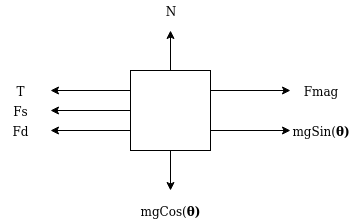
\includegraphics[width=0.8\linewidth]{imgs/FBD.png}
	\caption{Free-body diagram of forces acting upon the ball}%
	\label{fig:14}
\end{figure}

Forces on x-axis : \\
\[
Fmag + mg + \sin (\theta ) - T - Fspring - Fdamper = m \ddot x \label{eq:1} \tag{\ding{1}}
\]
Forces on y-axis: \\
$N - mg\cos(\theta) = 0$  - (2)

Moment of inertia, i = $2/5mr^2$

Torque $M = -Tr$          (-Ve as rotating clockwise)

$I\ddot \theta = -Tr \rightarrow  1/2 mr^\cancel{2} \ddot\theta = -T\cancel{r}$

$T = -1/2 mr\ddot\theta$ 

By 'Pizza slice theorem', $\ddot x = \ddot \theta r$

Therefore, 
$T = 1/2 m \ddot x$ \\


Using python's symbolic differentiation, SymPy, to confirm the partial derivatives of {$\phi$} , {$\psi$} . 
\\
Equilibrium point is represented as $x_{1}^e, x_{2}^e, x_{3}^e, x_{4}^e, F^e = (0, 0, 0, 0, 0)$ \\

$
\begin{equations} \label{phi_differentials}
\frac{\delta \Phi \left ( F, x_{3}, x_{4} \right )}{\delta F}_{F^e, x_{3}^e, x_{4}^e} = \frac{4}{4 M + m} \\
\frac{\delta \Phi \left ( F, x_{3}, x_{4} \right )}{\delta x_{3}}_{F^e, x_{3}^e, x_{4}^e} = - \frac{3 g m}{4 M + m} \\
\frac{\delta \Phi \left ( F, x_{3}, x_{4} \right )}{\delta x_{4}}_{F^e, x_{3}^e, x_{4}^e} =   0 
\end{equations}
\\
\\
\begin{equations} \label{psi_differentials}
\frac{\delta \psi \left ( F, x_{3}, x_{4} \right )}{\delta F}_{F^e, x_{3}^e, x_{4}^e} = - \frac{3}{\ell \left(4 M + m\right)} \\
\frac{\delta \psi \left ( F, x_{3}, x_{4} \right )}{\delta x_{3}}_{F^e, x_{3}^e, x_{4}^e} = \frac{3 g \left(M + m\right)}{\ell \left(4 M + m\right)}\\
\frac{\delta \psi \left ( F, x_{3}, x_{4} \right )}{\delta x_{4}}_{F^e, x_{3}^e, x_{4}^e} =   0 
\end{equations}
$
